\usepackage{algorithmicx}\chapter{Modélisation des besoins énergétiques du quartier DISTRISIM}


    \begin{figure}[htp]
        \centering
        {\fbox{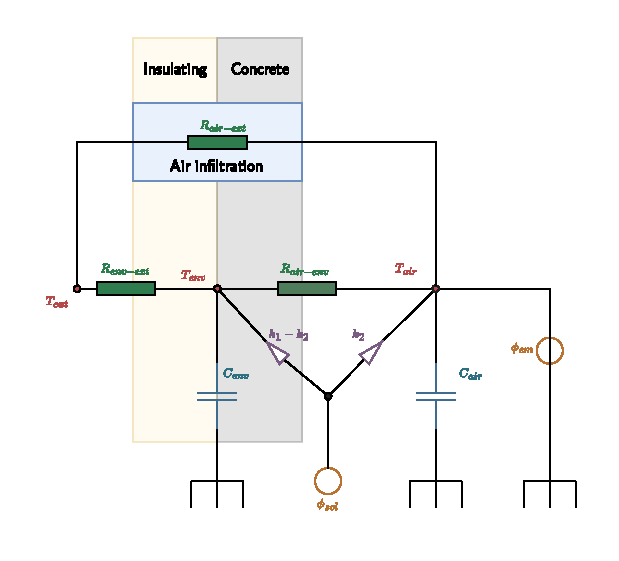
\includegraphics[width = 0.8\textwidth]{figures/diagrammes/schémas/DISTRISIM AE.drawio}}}
        \caption{Modèle RC utilisé pour modéliser un bâtiment DISTRISIM \textit(tiré de \cite{TST} et inspiré de \cite{aoun})}
    \end{figure}

    \section{Optimisation des paramètres du modèle}
        \subsection{Optimisation par essaims particulaires (PSO)}
            \cite{NIA}

            \cite{gad_particle_2022}

            \cite{yt_pso}

            \begin{algorithm}
                \caption{Optimisation par essaim de particules (PSO)}\label{alg:pso}
                \begin{algorithmic}
                    \Require
                    \Ensure
                    \State
                \end{algorithmic}
            \end{algorithm}

            \cite{TST}

            \begin{figure}[H]
                \centering
                    \subfloat[Température d'air intérieur, $RMSE = 0.55^ \circ \bf C$]{\fbox{
                        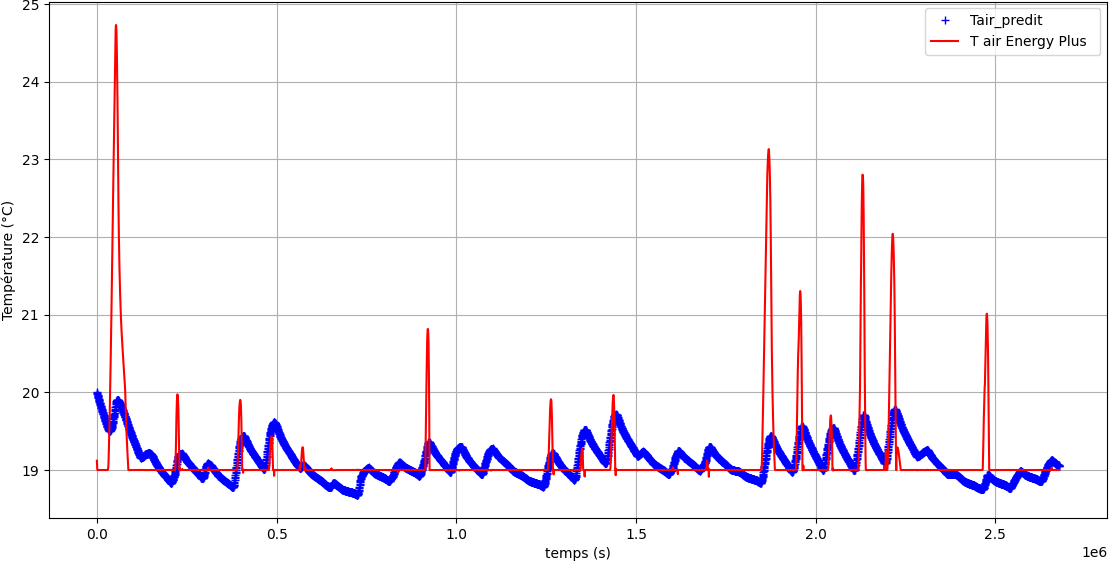
\includegraphics[width = 0.4\textwidth]{figures/diagrammes/courbes/TST_air_predit_VS_energyplus}}}\qquad
                    \subfloat[Besoins de chauffage, $RMSE = 16.31 \bf kW$]{\fbox{
                        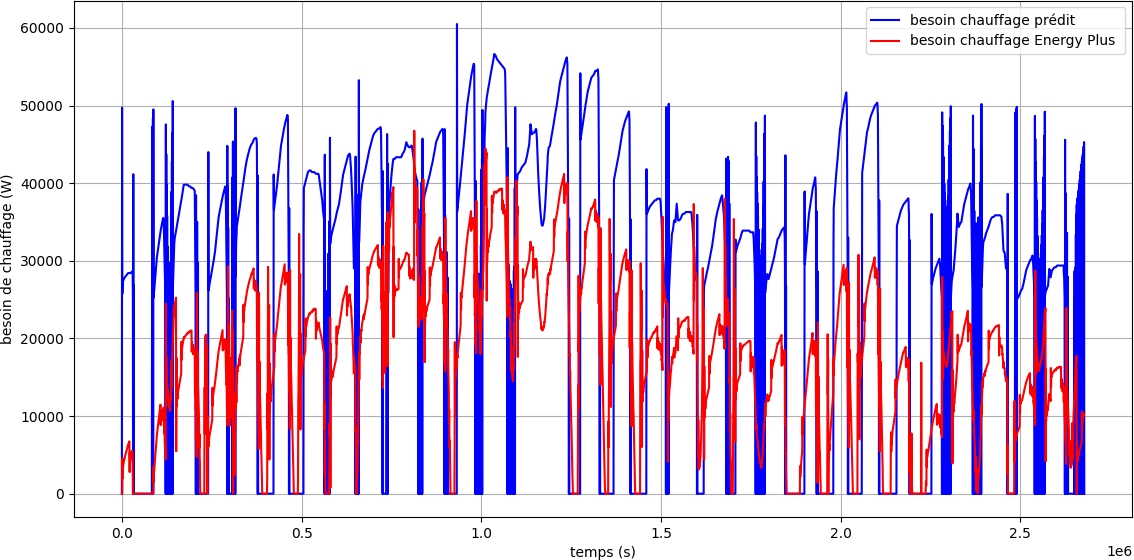
\includegraphics[width = 0.4\textwidth]{figures/diagrammes/courbes/TST_besoin_chauffage_VS_energyplus}}}\qquad
                \caption{Comparaison entre les modélisations d'Energy Plus et les prévisions du précédent stage \textit{(Bâtiment Thales)}}

            \end{figure}

    \section{}

        \cite{numerical_analysis}

        \begin{algorithm}
            \caption{Méthode de la sécante}\label{alg:sec}
            \begin{algorithmic}
                \Require
                \Ensure
                \State
            \end{algorithmic}
        \end{algorithm}
